\documentclass{beamer}
\usepackage{etex}
\usepackage{beamerthemesplit}
\usepackage{epstopdf}
\usepackage{hyperref}
\usepackage{verbatim} 
\usepackage{amsthm,amssymb,amsmath,graphicx}

\usepackage{multirow}
\usepackage{graphicx,subfigure}
\usepackage{amsmath,mathtools,amsthm}
\usepackage{pstricks,pst-node,pst-plot,pstricks-add,pst-grad,pst-slpe,overpic}
%\usepackage{epstopdf}
\usepackage{caption,verbatim}

\usepackage{mathptmx}
\usepackage{helvet}

\title{ Inverse Problem for Non-Viscous Mean Field Control: Example from Traffic}
\author{Shaurya Agarwal, Ph.D. Candidate}
\date{June 5, 2015}
\setbeamercolor{uppercol}{fg=white,bg=black}%
\setbeamercolor{lowercol}{fg=black,bg=white}%
\mode<presentation>
{
  \usetheme{Warsaw}
  \setbeamercovered{transparent}
}
\usefonttheme{serif}

\begin{document}

\begin{frame} % Cover slide
\titlepage
\begin{center}
{\color{red} \large {\textsc{Transportation Research Center}}}\\

\vspace{2mm}


\includegraphics[scale=0.5]{UNLVRed}
\end{center}
\end{frame}

%\section[Acknowledgement]{}
\frame{
\frametitle{Acknowledgement}
\begin{itemize}[<+->]
\item I would like to express my sincere thanks and gratitude to my advisors, Dr. Monika Neda and Dr. Pushkin Kachroo, who have supported and motivated me throughout my thesis.
\item I am also highly grateful to all my committee members, Dr. Amei Amei, Dr. Dieudonne Phanord and Dr. Anjala Krishen for their time and insightful remarks.

\item I am also thankful to all the friends and colleagues at Transportation Research Center for their help and support.
\end{itemize}
}
\frame{
\frametitle{Outline of the Presentation}
\begin{itemize}[<+->]
\item Contribution
\item Introduction and Motivation
\item Mathematical Background
\item Inverse Derivation of LWR Model for Traffic
\item Inverse Derivation of Travel Time PDE for Traffic
\item Stationary Mean Field Games and Traffic
\item Future Work and Conclusion
\end{itemize}
}



%\section{Contribution}

%\frame{\tableofcontents}
\frame{
\frametitle{Contributions}
\begin{itemize}
\item<1-> We derive the traffic dynamics (LWR Model) solving an inverse problem, which provides a link between the microscopic behavior of drivers to the macroscopic behavior of traffic.
\item<2-> The travel time dynamics is derived linking the  driver behavior to the evolved traffic behavior.
\item<3-> To our best knowledge, Mean Field Games framework has not been used before to derive the fundamental LWR traffic dynamics and the Travel time dynamics.
\item<4-> This connection between the microscopic and macroscopic behavior can lead researchers to design traffic controllers from both sides.
\end{itemize}
}


\section{Introduction and Motivation}
\frame{
\begin{center}
 {\large Introduction and Motivation}
\end{center}
}
\subsection[Introduction and Motivation]{}
%\frame{\tableofcontents}
\frame{
\frametitle{Introduction and Motivation}
\begin{itemize}
\item<1-> {M}{ean} field games (MFG) involve the study of Nash equilibrium among infinitely many players where the interplay is between individual dynamics and the continuum limit of the players.
\item<2-> Mean field framework has been used in many applications such as consensus building, complex networks, electric vehicles using smart grid.
\item<3-> There has been some work in utilizing the mean field principles in transportation problems in one (vehicular traffic) and two dimensions (pedestrian traffic).
\end{itemize}
}

\frame{
\frametitle{Introduction and Motivation (contd..)}

\begin{itemize}[<+->]
\item Vehicular traffic on the highways can be viewed microscopically, i.e. in terms of each vehicle, or macroscopically, i.e. in terms of aggregate variables such as traffic density and flow.
\item The microscopic dynamics of vehicles such as the car-following models, result in the evolution of macroscopic dynamics, such as the LWR (Lighthill Whitham Richards) model.
\end{itemize}
}

%\subsection{Work Done}
%\frame{
%\frametitle{Background}
%\begin{itemize}
%  \item We derive the traffic dynamics solving an inverse problem providing a link between the microscopic behavior of drivers to the macroscopic behavior of traffic.  
%  \item This is similar to how Newton's laws and other physical fundamental laws for instance are derived from variational principles of mechanics.  
%  \item We further utilize the recently developed framework of the mean field games to connect the optimizing behavior of the drivers to the evolving macroscopic traffic behavior.
%  \item  To our knowledge, this framework has not been used before to derive the fundamental LWR traffic dynamics. 
%  \item The travel time dynamics is being used to link driver behavior to the evolved traffic behavior for the first time. 
%  \item This connection between the microscopic and macroscopic behavior can lead researchers to design traffic controllers from both sides.
%\end{itemize}
%}

%%%%%%%%%%%%%%%%%%------------->>>>>>>>>>>>>>>>>>>

%\section[Mathematical Background]{}
\frame{
\begin{center}
\begin{large}
Mathematical Background
\end{large} 
\end{center}
}

\subsection{Mean Field Games}
\frame{
\frametitle{Mean Field Games: Agent Model}
We consider agent stochastic differential model on a probability space $(\Omega, \mathcal{A},P)$ with a filtration $\mathcal{F}^t$ generated by $w(t)$, the $n$-dimensional standard Wiener process

\begin{equation}\label{eqn:AgentModel}
\begin{multlined}
dx=v(x(t),u(x(t)),\rho(x,t))dt+\sigma(x(t)) dw(t), \\
x(0)=x_0,
\end{multlined}
\end{equation}
\noindent where $v : \mathcal{R}^n \times \mathcal{R}^d \times \mathcal{R}^n \to \mathcal{R}^n$, and $\sigma : \mathcal{R}^n \to \mathcal{L}(\mathcal{R}^n;\mathcal{R}^n)$ are measurable functions, $\rho$ is the probability density of the state $x(t)$, and $u(x(t))$ is the state feedback control.
}

\frame{
\frametitle{Mean Field Games: Value Function}
The objective for the control law design for the agent is the expected cost for a given initial condition $x$ and time $t$.
\begin{equation}\label{eqn:AgentModelCost}
\begin{multlined}
J_{x,t}[u(\cdot)]= E\left\lbrace \int_t^T r(x(s),u(x(s)),\rho(s))ds + k(x(T)) \right\rbrace ,
\end{multlined}
\end{equation}

\noindent where, $r$ and $k$ are known functions representing the running cost and the terminal cost respectively.

The value function for this problem is
\begin{equation}\label{eqn:AgentModelValue}
\mathcal{V}(x,t)=\displaystyle \inf_{u(\cdot) \epsilon \: \mathcal{U}}J_{x,t}[u(\cdot)].
\end{equation}
}

\frame{
\frametitle{Mean Field Games: Coupled PDE System}

\begin{block}{PDE satisfied by the value function is stochastic HJB Equation}
\begin{equation}\label{eqn:SHJB}
\begin{multlined}
\mathcal{V}_t(x,t)+\frac{\sigma^2}{2}\Delta \mathcal{V}(x,t)+
\displaystyle \min_{u(\cdot) \epsilon \: \mathcal{U}}\left\lbrace v(x,u,\rho,t)\nabla_x\mathcal{V}(x,t) + r(x,u) \right\rbrace =0, \\
\mathcal{V}(x,T)=k(x).
\end{multlined}
\end{equation}
\end{block}

\begin{block}{Fokker Planck equation for the evolution of state probability density}
\begin{equation}\label{eqn:FP}
\begin{multlined}
\rho_t(x,t)-\frac{\sigma^2}{2}\Delta \rho(x,t)+
\nabla \cdot (\rho v(x,u,\rho,t)) =0, \\
\rho(x,0)=\rho_0(x).
\end{multlined}
\end{equation}
\end{block}

\eqref{eqn:SHJB} and \eqref{eqn:FP} form HJB-FP system or coupled PDE system of MFG.
}

%%%%%%%%--------------?>>>>>>>>>>>>>>>>>>>>>>>>>>>>>>>>>>
\subsection{Vanishing Viscosity Mean Field}

%\frame{
%\frametitle{Liouville Equation}
%Let the control system be described by
%\begin{equation}
%\dot{x}(t) = v(x(t),u(t)) \label{eqn:control_system}
%\end{equation}
%where $x = (x_1,\ldots,x_n)$ and $u$ is the control input. Then Liouville equation becomes:
%\begin{block}{Liouville Equation}
%\begin{equation}\label{eqn:LE-CS}
%\rho(x,t,u(\cdot))_t + [\rho(x,t,u(\cdot))v(x(t),u(t))]_x = 0.
%\end{equation}
%\end{block}
%
%The solution to the Liouville equation can be obtained by the method of characteristics.
%}

\frame{
\frametitle{Hyperbolic HJB and the Liouville equation}
Letting $\sigma \to 0$ in equation \eqref{eqn:SHJB} and equation \eqref{eqn:FP}, we get equations for vanishing viscosity Mean Field Games.
\begin{block}{Vanishing Viscosity Mean Field Games}
\begin{equation}\label{eqn:VSHJB}
\begin{multlined}
\mathcal{V}_t(x,t)+
\displaystyle \min_{u(\cdot) \epsilon \: \mathcal{U}}\left\lbrace v(x,u,\rho,t)\nabla_x\mathcal{V}(x,t) + r(x,u) \right\rbrace =0,\\
\mathcal{V}(x,T)=k(x),
\end{multlined}
\end{equation}

\begin{equation}\label{eqn:VFP}
\begin{multlined}
\rho_t(x,t)-\nabla \cdot (\rho v(x,u,\rho,t)) =0,\\
\rho(x,0)=\rho_0(x).
\end{multlined}
\end{equation}
\end{block}
The first equation is hyperbolic HJB and second one is the Liouville equation instead of the Fokker Planck one from before.
}

%%%%%%%%%%%%%%%%%%%%%%%%%%%%%%%%-->>>>>>>>>>>>>>>>>
\subsection{LWR Model for Traffic Dynamics}

\frame{
\frametitle{LWR and Greenshield's Models for Traffic}
 The dynamics of traffic flow using LWR model is given as

\begin{equation}\label{eqn:TrafficModel}
\rho_t (t,x) + f_x(t,x) = 0,
\end{equation}
\noindent where, $\rho$ is the traffic density and $f= \rho v$ is the flux. \\

Greenshield's model which proposes a linear relationship between traffic density and traffic speed is given as
\begin{equation}\label{eqn:TrafficModels:Greenshields}
v(\rho)=v_{f}\left( 1-\frac{\rho}{\rho_{m}}\right),
\end{equation}
\noindent where $v_{f}$ is the free flow speed and $\rho_{m}$ is the maximum possible density or jam density.  
}

\begin{frame}
\frametitle{LWR Model}
\scriptsize{
\begin{columns}
\begin{column}{4cm}
\begin{overprint}
\only<1>{\begin{beamerboxesrounded}[upper=uppercol,lower=lowercol,shadow=true,width=5cm]{Fundamental Diagram}
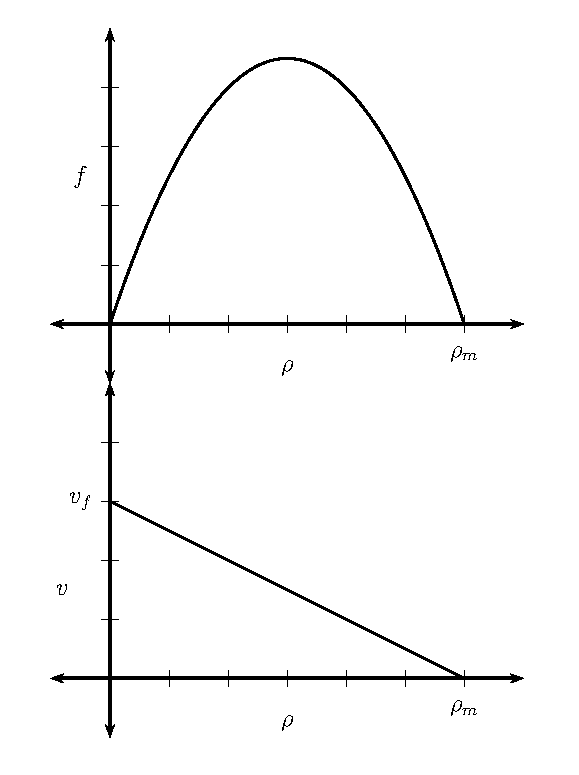
\includegraphics[scale=0.5]{Greenshield}
\end{beamerboxesrounded}
}
\only<2>{\begin{beamerboxesrounded}[upper=uppercol,lower=lowercol,shadow=true,width=5cm]{Fundamental Diagram}
\includegraphics[scale=0.5]{Greenberg}
\end{beamerboxesrounded}
}
\only<3>{
\begin{beamerboxesrounded}[upper=uppercol,lower=lowercol,shadow=true,width=5cm]{Fundamental Diagram}
\includegraphics[scale=0.5]{Underwood}
\end{beamerboxesrounded}
}
\end{overprint}
\end{column} 
\begin{column}{6cm}
\begin{block}{Conservation}
$$
\frac{\partial }{\partial t}\rho (t,x) + \frac{\partial }{\partial x}f(t,x) = 0
$$
$$
f = \rho (t,x) v(t,x)
$$
\end{block}
\only<1>{
\begin{exampleblock}{Greenshield Model}
\[ v(\rho)=v_{f}(1-\frac{\rho}{\rho_{m}}) \]
\end{exampleblock}
}
\only<2>{
\begin{exampleblock}{Greenberg Model}
\[ v(\rho)=v_{f}\,ln(\frac{\rho_m}{\rho}) \]
\end{exampleblock}
}
\only<3>{
\begin{exampleblock}{Underwood Model}
\[ v(\rho)=v_{f}\,\exp(\frac{-\rho}{\rho_{m}}) \]
\end{exampleblock}
}
%\only<4>{
%\begin{exampleblock}{Diffusion Model}
%\[ v(\rho)=v_{f}(1-\frac{\rho}{\rho_{m}})-\frac{D}{\rho}(\frac{\partial \rho}{\partial x}) \]
%\end{exampleblock}
%}
\end{column}
\end{columns}
}
\end{frame}

\begin{frame}
\frametitle{Characteristic Solution for Conservation Laws}
\begin{columns}
\begin{column}[c]{5cm}
\begin{beamerboxesrounded}[upper=uppercol,lower=lowercol,shadow=true]{Characteristic Slopes}
\includegraphics[scale=0.5]{ch_slopes}
\end{beamerboxesrounded}
\begin{beamerboxesrounded}[upper=uppercol,lower=lowercol,shadow=true]{Solution at Time t}
\includegraphics[scale=0.5]{soln}
\end{beamerboxesrounded}
\end{column}
\begin{column}[c]{5cm}
\begin{beamerboxesrounded}[upper=uppercol,lower=lowercol,shadow=true]{Characteristic Speed}
\includegraphics[scale=0.5]{FD_slope}
\end{beamerboxesrounded}
\begin{beamerboxesrounded}[upper=uppercol,lower=lowercol,shadow=true]{Solution Blowup}
\includegraphics[scale=0.5]{ch_intersect}
\end{beamerboxesrounded}
\end{column}
\end{columns}
\end{frame}
%----------------------------------------------------------SLIDE -
\begin{frame}
\frametitle{Characteristics}
\begin{beamerboxesrounded}[upper=uppercol,lower=lowercol,shadow=true,width=6cm]{Initial Conditions Propagations}
\includegraphics[scale=0.5]{prop}
\end{beamerboxesrounded}
\end{frame}
%----------------------------------------------------------SLIDE -
\begin{frame}
\frametitle{Distributional Solution}
\begin{block}{Cauchy Problem}
$$
u_t + f(u)_x = 0 
$$
$$
u(0,x)=u_0(x)
$$
\end{block}
\begin{alertblock}{Distributional Solution}
A measurable locally integrable function $u(t,x)$ is a solution in the distributional sense of the Cauchy problem if for every test function $\phi$
\begin{eqnarray}
\iint_{R^+ \times R}[u(t,x)\,\phi_{t}(t,x) + f(u(t,x))\,\phi_{x}(t,x)]\;dx\,dt + \int_{R} u_{0}(x)\,\phi(x,0)\;dx=0 \nonumber
\end{eqnarray}
\end{alertblock}
\end{frame}
%----------------------------------------------------------SLIDE -
\begin{frame}
\frametitle{Weak Solution}
\begin{block}{Weak Solution}
Distributional solution in the open strip; initial condition, $L^1$ cont. in t
$$
u(t,x) = u(t,x^+)
$$
$$
\mathop {\lim }\limits_{t \to 0} \int_R \left|u(t,x)-u_0(x)\right|dx = 0
$$
\end{block}
\end{frame}
%----------------------------------------------------------SLIDE -
\begin{frame}
\frametitle{Shock Wave in Scalar Riemann Problems}
\scriptsize{
\begin{columns}
\begin{column}[c]{5cm}
\begin{beamerboxesrounded}[upper=uppercol,lower=lowercol,shadow=true,width=4cm]{Shock Characteristics}
\includegraphics[scale=0.6]{shock}
\end{beamerboxesrounded}
\end{column}
\begin{column}[c]{5cm}
\begin{beamerboxesrounded}[upper=uppercol,lower=lowercol,shadow=true,width=4cm]{Shock Speed}
\includegraphics[scale=0.6]{shockSp}
\end{beamerboxesrounded}
\end{column}
\end{columns}
\begin{exampleblock}{Calculating Shock Speed}
\begin{eqnarray*}
\lambda (\rho_r - \rho_{\ell}) = f(\rho_r) - f(\rho_{\ell})
\end{eqnarray*}
\end{exampleblock}
}
\end{frame}
%----------------------------------------------------------SLIDE -
\begin{frame}
\frametitle{Rarefaction Wave}
\scriptsize{
\begin{columns}
\begin{column}[c]{6cm}
\begin{beamerboxesrounded}[upper=uppercol,lower=lowercol,shadow=true,width=6cm]{Blank Region}
\includegraphics[scale=0.6]{blank}
\end{beamerboxesrounded}
\end{column}
\begin{column}[c]{5cm}
\begin{beamerboxesrounded}[upper=uppercol,lower=lowercol,shadow=true,width=4cm]{Entropy Violating Solution}
\includegraphics[scale=0.6]{EntVio}
\end{beamerboxesrounded}
\end{column}
\end{columns}
\begin{beamerboxesrounded}[upper=uppercol,lower=lowercol,shadow=true,width=10cm]{Rarefaction Solution}
\includegraphics[scale=0.6]{rare}
\end{beamerboxesrounded}}
\end{frame}
%----------------------------------------------------------SLIDE -
\begin{frame}
\frametitle{Admissibility Conditions}
\scriptsize{
\begin{columns}
\begin{column}[c]{4cm}
\begin{block}{Vanishing Viscosity}
\[
	u_t^{\epsilon} + f(u^{\epsilon})_x = \epsilon u_{xx}^{\epsilon}
\]
\end{block}
\end{column}
\begin{column}[c]{4cm}
\begin{block}{Entropy}
\[
\frac{\partial \eta(u)}{\partial t} + \frac{\partial q(u)}{\partial x} \leq 0
\]
\end{block}
\end{column}
\end{columns}
\begin{block}{Lax Admissibility Condition}
\[
\lambda(u_{\ell}) \geq \lambda \geq \lambda(u_r)
\]
\end{block}
\begin{alertblock}{Kruzkov's Entropy Function}
\[
\eta(u) = \left|u - k\right| \mbox{ and } q(u) = sign(u - k)\cdot(f(u) - f(k))
\]
\[
\int\!\int_{\Pi_T} \{ |u(x,t)-k|\phi_t+\mathop{\rm sign}(u(x,t)-k)[f(x,t,
u(x,t))-f(x,t,k)]\phi_x
\]
\[
-\mathop{\rm sign}(u(x,t)-k)[f_x(x,t, u(x,t))-g(x,t, u(x,t))]\}dxdt\geq 0  \]

\[
\lim_{t\to 0}\int_{K_r}|u(x,t)-u_0(x)|dx=0.
\]
\end{alertblock}
}
\end{frame}


%%%%%%%%%%%%--------------------------------->>>>>>>>>>>>>>

\section{Derivation of LWR and Greenshield's Model}

\frame{
\begin{center}
{\large Derivation of LWR and Greenshield's Model using Mean Field Framework} 
\end{center}
}

\frame{
\frametitle{Problem Setup}
We take the agent model to be
\begin{equation}\label{eqn:MAgentModel}
\begin{multlined}
dx=u(t)dt+\sigma(x(t)) dw(t), \: \: x(0)=x_0.
\end{multlined}
\end{equation}

Define a function $h(x(t),t)$ as 
\begin{equation}
h: = - \frac{v_f}{2} (1- \frac{\rho(x(t), t)}{\rho_m}),
\end{equation}
\noindent where $v_f$ is the traffic free flow speed, $\rho_m$ is the traffic jam density and $\rho(x(t), t)$ is the density at time $t$ and position $x$.
}

\frame{
\frametitle{Problem Setup}
Now we define the running cost $r(x(t), t, u(t))$ as 
\begin{equation}
r(x(t), t, u(t)): =  \frac{1}{2} u^2 (t),
\end{equation}
\noindent where $u(t)$ is the control variable and the cost function as

\begin{equation}\label{eqn:MAgentModelCost}
\begin{multlined}
J_{x,t}[u(\cdot)]= 
E\left\lbrace \int_{t}^{t_f} r(x(s),s,u(s))ds + \int_{x}^{x_f} h(x(s),s) ds \right\rbrace,
\end{multlined}
\end{equation}
}

\subsection{Derivation of the Greenshield's Model}
\frame{
\frametitle{Inverse Derivation of the Greenshield's Model}
\begin{lemma}[Inverse Derivation of the Greenshield's Model]\label{lemma:GM}
For the stochastic differential equation model given by  \eqref{eqn:MAgentModel} the optimal control for the cost function given by \eqref{eqn:MAgentModelCost} is given by 
\begin{equation}
u(t) = v_f (1- \frac{\rho}{\rho_m}).
\end{equation}
\end{lemma}
}

\frame{
\frametitle{Proof}
The value function for the system given by equation \eqref{eqn:MAgentModel} whose cost function is given by equation \eqref{eqn:MAgentModelCost} is 

\begin{equation}
\begin{multlined}
\mathcal{V}(x(t),t) = 
\min_{u(\cdot)} E\left\lbrace \int_{t}^{t_f} r(x(s),s,u(s))ds + \right. 
\left. 
\int_{x}^{x_f} h(x(s),s) ds \right\rbrace.
\end{multlined}
\end{equation}

By subdividing the interval we obtain

\begin{equation}
\begin{multlined}
\mathcal{V}(x(t),t) = \min_{u(\cdot)} 
E\left\lbrace  
\int_{t}^{t+\Delta t} r d\tau + \int_{t + \Delta t}^{t_f} r d\tau+ 
\right. 
\left. 
\int_{x}^{x+ \Delta x} h ds + \int_{x+ \Delta x}^{x_f} h ds \right\rbrace .
\end{multlined}
\end{equation}

}

\frame{
The principle of optimality requires that

\begin{equation}
\begin{multlined}
\mathcal{V}(x(t),t) = \min_{u(t)} 
E\left\lbrace  
\int_{t}^{t+\Delta t} r d\tau + \int_{x}^{x+ \Delta x} h ds + 
\right. 
\left. 
\mathcal{V}(x+\Delta x,t +\Delta t)  \vphantom{\frac{\sigma^2}{2}}
\right\rbrace ,
\end{multlined}
\end{equation}

\noindent where $\mathcal{V}(x+\Delta x,t +\Delta t)$ is the minimum value of the process for the time interval $t+ \Delta t < \tau < t_f$, and with initial state $x(t+ \Delta t	)$.
}

\frame{
Expanding $\mathcal{V}(x+\Delta x,t +\Delta t)$ using Ito's chain rule about the point $(x(t), t)$

\begin{equation}
\begin{multlined}
\mathcal{V}(x(t),t) = \min_{u(t)} 
E\left\lbrace  
\int_{t}^{t+\Delta t} r d\tau + \int_{x}^{x+ \Delta x} h ds + 
\right. 
\left.
\mathcal{V}(x(t),t) + \right. \\
\left.
\left[\mathcal{V}_t (x(t),t)+ \frac{\sigma^2}{2}\Delta \mathcal{V}(x(t),t)\right]\Delta t + \nabla_x\mathcal{V}(x(t),t)\Delta x + \mbox{h.o.t.}  \vphantom{\frac{\sigma^2}{2}}
\right\rbrace ,
\end{multlined}
\end{equation}
For small  $\Delta t$ we can write

\begin{equation}
\begin{multlined}
\mathcal{V}(x(t),t) = \min_{u(t)} 
E\left\lbrace  
r\Delta t + h\Delta x + \mathcal{V}(x(t),t) + 
\vphantom{\frac{\sigma^2}{2}}
\right. 
\left. 
\bigg [ \mathcal{V}_t (x(t),t)+
\right.   \\
\left. \left.
\frac{\sigma^2}{2}\Delta \mathcal{V}(x(t),t) + \nabla_x\mathcal{V}(x(t),t)u(t)  \vphantom{\frac{\sigma^2}{2}}\right ] \Delta t + \mbox{h.o.t.}  \vphantom{\frac{\sigma^2}{2}}
\right\rbrace,
\end{multlined}
\end{equation}
}

\frame{
\noindent Substituting  $\Delta x = u(t) \Delta t$, dividing by $\Delta t$ and letting $\Delta t \to 0$ yields

\begin{equation} \label{eqn:HJB}
\begin{multlined}
0 = \mathcal{V}_t (x(t),t)+\min_{u(t)} 
E\left\lbrace  
r + hu(t) + 
\vphantom{\frac{\sigma^2}{2}}
\right.  
\left. 
\frac{\sigma^2}{2}\Delta \mathcal{V}(x(t),t) + \nabla_x\mathcal{V}(x(t),t)u(t)  
\right\rbrace .
\end{multlined}
\end{equation}

Define the Hamiltonian $\mathcal{H}$ as

\begin{equation} \label{eqn:hamiltonian}
\mathcal{H} =  
r + hu(t) + \nabla_x\mathcal{V}(x(t),t)u(t)  + \frac{\sigma^2}{2}\Delta \mathcal{V}(x(t),t).
\end{equation}

Using \eqref{eqn:HJB} and \eqref{eqn:hamiltonian} we obtain the stochastic Hamilton-Jacobi equation as

\begin{equation}
\boxed {0  = \mathcal{V}_t (x(t),t)  + \mathcal{H}^* }.
\end{equation}
}
%%%%%%%
\frame{To calculate the optimal value of the control $u(t)$, we differentiate $\mathcal{H}$ with respect to $u(t)$ and equate to zero

\begin{equation}
\begin{multlined}
\frac{\partial \mathcal{H}}{\partial u} = 
\frac{\partial}{\partial u} \left[ \frac{1}{2}u^2(t) + hu(t) + \frac{\sigma^2}{2}\Delta \mathcal{V}(x(t),t) + 
\right.  
\left. 
\vphantom{\frac{\sigma^2}{2}}
\nabla_x\mathcal{V}(x(t),t)u(t)   \right] = 0.
\end{multlined}
\end{equation}

\noindent This gives the control law $u(t)$ as

\begin{equation}
u(t) = - (\nabla_x\mathcal{V}(x(t),t) + h).
\end{equation}
\noindent Now replacing the values of $\nabla_x\mathcal{V}(x(t),t)$ and $h$ in the above equation yields Greenshield's traffic flow formula,

\begin{equation}
\boxed{u(t) = v_f (1- \frac{\rho}{\rho_m}).}
\end{equation}
}

\subsection{Mean Field Game Equations}
\frame{
\frametitle{Mean Field Game Equations}
Putting $u(t)$ in equation \eqref{eqn:HJB} we obtain the HJB equation as
\begin{block}{}
\begin{equation} \label{eqn:HJB1}
\begin{multlined}
0 = \mathcal{V}_t (x(t),t)+
\frac{\sigma^2}{2}\Delta \mathcal{V}(x(t),t) + v_f (1- \frac{\rho}{\rho_m})\nabla_x\mathcal{V}(x(t),t).
\end{multlined}
\end{equation}   
\end{block}


\noindent The Fokker Planck equation for the evolution of the probability density function (pdf) of the state is given by
\begin{block}{}
\begin{equation} \label{eqn:FPK1}
\begin{multlined}
\rho_t(x,t)-\frac{\sigma^2}{2}\Delta \rho(x,t)+
\nabla \cdot (\rho v(x,u,\rho,t)) =0,\\
\rho(x,0)=\rho_0(x).
\end{multlined}
\end{equation}
\end{block}

                
Equations \eqref{eqn:HJB1} and \eqref{eqn:FPK1} represent the coupled PDE system of the Mean Field Games.
}

%%%%%%%->>>>>>>>>>>>>.
\subsection{Derivation of the LWR Model}
\frame{
\frametitle{Derivation of the LWR Model}
\begin{theorem}[Inverse Derivation of the LWR Model]\label{theorem:Inv}
For the stochastic differential equation model given by equation \eqref{eqn:MAgentModel} the vanishing viscosity solution for the mean field game for the cost function given by equation \eqref{eqn:MAgentModelCost} is the LWR model
\begin{equation}
\rho_t+f_x(\rho)=0
\end{equation} 
\noindent where, $f=\rho v$ and 
\begin{equation}
v(\rho) = v_f (1- \frac{\rho}{\rho_m})
\end{equation}
\end{theorem}
}
%%
\frame{
\frametitle{Proof}
Lemma \ref{lemma:GM} showed that the optimal control, which is the vehicle speed for  the stochastic model given by equation \eqref{eqn:MAgentModel} is 
\begin{equation}
v(\rho) = v_f (1- \frac{\rho}{\rho_m}).
\end{equation}

Moreover, the Fokker Planck equation for the evolution of the pdf of the state is given by

\begin{equation}
\begin{multlined}
\rho_t(x,t)-\frac{\sigma^2}{2}\Delta \rho(x,t)+
\nabla \cdot (\rho v(x,u,\rho,t)) =0,\\
\rho(x,0)=\rho_0(x).
\end{multlined}
\end{equation}

Letting $\sigma \to 0$ gives us the conservation law of the LWR model.
}

%%%%%%%%%%%%%%%------------->>>>>>>>>>>>>>>>>>>>>>>>>>>>>>>>>>>>>>>>>>>>>
\section{Derivation of Travel Time PDE}
\frame{
\begin{center}
{\large Travel Time Dynamics using HJB equation and Pontryagin's Minimization Principle }
\end{center}
}

\frame{
\frametitle{Travel Time Dynamics}

\begin{block}{Theorem: Travel Time PDE}
Expected value of the travel time $T(x(t), t)$ of the agent to a fixed location is given as:
\begin{equation}
T_t(x,t) + T_x(x,t)v(\rho) + 1 = 0.
\end{equation}
\end{block}
}

\subsection{Problem Formulation}
\frame{
\frametitle{Problem Setup}

Take the agent model once again to be
\begin{equation}\label{eqn:TTAgentModel}
\begin{multlined}
dx=u(t)dt+\sigma(x(t)) dw(t), \: \: x(0)=x_0.
\end{multlined}
\end{equation}

Define the cost function to be the expected value of the travel time $T(x(t), t)$ of the agent to a fixed location,

\begin{equation}\label{eqn:TTAgentModelCost}
\begin{multlined}
J_{x,t}[u(\cdot)]= E\{T(x(t), t)\}.
\end{multlined}
\end{equation}

The value function for the problem becomes

\begin{equation}
\mathcal{V}(x(t), u(t),  t) = \min_{u(t)} E\left \{ T(x(t), t) \right \}.
\end{equation} 
}

\subsection{Proof}
\frame{
\frametitle{Proof}
By subdividing the interval we obtain

\begin{equation}
\mathcal{V}(x(t), t) = \min_{u(t)} E\left \{ \Delta t + \mathcal{V}(x(t + \Delta t), t+ \Delta t)  \right \},
\end{equation}

\noindent where $\mathcal{V}(x+\Delta x,t +\Delta t)$ is the minimum expected travel time of the process for the time interval $t+ \Delta t < \tau < t_f$, and with initial state $x(t+ \Delta t)$.

Expanding $\mathcal{V}(x+\Delta x,t +\Delta t)$ using Ito's chain rule about the point $(x(t), t)$

\begin{equation}
\begin{multlined}
\mathcal{V}(x(t), t) = \min_{u(t)} E\left \{ \Delta t + \mathcal{V}(x(t), t) + 
\vphantom{\frac{\sigma^2}{2}}
\right.  
\left. 
\mathcal{V}_t \Delta t + \mathcal{V}_x \Delta x +\frac{\sigma^2}{2} \Delta \mathcal{V}\Delta t + h.o.t.  \right \}.
\end{multlined}
\end{equation}
}


\frame{
\frametitle{}
Simplifying and canceling $\mathcal{V}(x(t), t)$ from both sides we get

\begin{equation}
\begin{multlined}
0 = \min_{u(t)} E\left \{ \Delta t + \mathcal{V}_t \Delta t + \mathcal{V}_x u(t)\Delta t +
\vphantom{\frac{\sigma^2}{2}}
\right.  
\left. 
\frac{\sigma^2}{2} \Delta \mathcal{V}\Delta t + h.o.t.  \right \}.
\end{multlined}
\end{equation}

Now dividing by $\Delta t$ and taking the limit as $\Delta t \to 0$ we get

\begin{equation}
0 = \min_{u(t)} \left \{ 1  + \mathcal{V}_t + \mathcal{V}_x u(t)+\frac{\sigma^2}{2} \Delta \mathcal{V} \right \}.
\end{equation}
}

\frame{
\frametitle{}
Now define the Hamiltonian $\mathcal{H}$ as

\begin{equation}
\mathcal{H}^*: = \min_{u(t)} \left \{ 1  + \mathcal{V}_xu(t)  \right \}.
\end{equation}

The stochastic Hamilton-Jacobi-Bellman equation then becomes

\begin{equation}
\boxed{0  = \mathcal{V}_t + \frac{\sigma^2}{2} \Delta \mathcal{V}+\mathcal{H}}^*.
\end{equation}
}

\frame{
\frametitle{}
\begin{itemize}
\item Pontryagin's minimum principle asks to minimize $\mathcal{H}$ as a function of $u \in [0, v_f(1- \rho/\rho_m)]$ at each fixed time $t$
\item Since $\mathcal{H}$ is linear in $u$, it follows that the minimum occurs at one of the endpoints $u = 0$ or $u = v_f(1- \rho/\rho_m)$, hence the control is bang-bang
\item Since $\mathcal{V}_x$ is negative (travel time value decreases as a function of $x$), hence to minimize the travel time we choose the maximum possible speed, which is

\begin{equation}
u(t) = v(\rho) = v_f(1- \frac{\rho}{\rho_m}).
\end{equation}
\end{itemize}
The dynamics of the expected travel time are given by the PDE

\begin{equation}
\mathcal{V}_t + \mathcal{V}_x u(t)+\frac{\sigma^2}{2} \Delta \mathcal{V} + 1 = 0.
\end{equation}
}

\frame{
\frametitle{}
Replacing the value of optimal control $u(t)$ in the above equation yields
\begin{block}{HJB equation for expected travel time}
\begin{equation} \label{eqn:HJB2}
T_t + v_f(1- \frac{\rho}{\rho_m}) T_x  +\frac{\sigma^2}{2} \Delta T + 1 = 0,
\end{equation}
\end{block}
\noindent  and the Fokker Planck equation for the evolution of the pdf of the state is given by
\begin{block}{Fokker Plank Equation}
\begin{equation} \label{eqn:FPK2}
\begin{multlined}
\rho_t(x,t)-\frac{\sigma^2}{2}\Delta \rho(x,t)+
\nabla \cdot (\rho v(x,u,\rho,t)) =0,\\
\rho(x,0)=\rho_0(x).
\end{multlined}
\end{equation}
\end{block}
Equations \eqref{eqn:HJB2} and \eqref{eqn:FPK2} represent the coupled PDE system for the Mean Field Games.
}

\frame{
\frametitle{}
Now in the case of vanishing viscosity $(\sigma \to 0)$ equation \eqref{eqn:HJB2} becomes the PDE shown here, for the travel time field.

\begin{block}{Travel Time PDE}
\begin{equation}
T_t(x,t) + T_x(x,t)v(\rho) + 1 = 0.
\end{equation}
\end{block}
}

%%%%%%%%%%%%%%%----------->>>>>>>>>>>>>>>>>>>>>>>>>>>>>>>>>>>>>>>>>>>>>>>>>.
\section{Stationary Mean Field Games}
\frame{
\frametitle{}
\begin{center}
{\large Stationary Mean Field Games and Traffic Theory}
\end{center}
}

\subsection{Stationary MFG for LWR Model}

\frame{
\frametitle{Stationary MFG Equations}
Stationary HJB equation for inverse problem of deriving LWR model is given as

\begin{equation} \label{eqn:HJB_st_1}
\begin{multlined}
\frac{\sigma^2}{2}\frac{d^2}{dx^2} \mathcal{V}(x) + v_f (1- \frac{\rho}{\rho_m})\frac{d}{dx}\mathcal{V}(x) = 0,
\end{multlined}
\end{equation}

The corresponding stationary FPK equation is given as

\begin{equation} \label{eqn:FPK_st_1}
\begin{multlined}
-\frac{\sigma^2}{2}\frac{d^2}{dx^2} \rho(x)+
\frac{d}{dx}(\rho v(\rho)) = 0.
\end{multlined}
\end{equation}
}

\frame{
\frametitle{Position Invariants}
Equation (\ref{eqn:HJB_st_1}) produces the following position invariant ($K_1$),

\begin{equation} \label{eqn:HJB_st_1_inv}
\begin{multlined}
\frac{\sigma^2}{2}\frac{d}{dx} \mathcal{V}(x) + v_f (1- \frac{\rho}{\rho_m})\mathcal{V}(x) = K_1.
\end{multlined}
\end{equation}

Similarly, equation (\ref{eqn:FPK_st_1}) produces the following position invariant ($K_2$),

\begin{equation} \label{eqn:FPK_st_1_inv}
\begin{multlined}
-\frac{\sigma^2}{2}\frac{d}{dx} \rho(x)+
\rho v(\rho) = K_2.
\end{multlined}
\end{equation}
}

\frame{
\frametitle{Existence of Unique Solutions}
Equations \eqref{eqn:HJB_st_1_inv} and \eqref{eqn:FPK_st_1_inv} can be rearranged as follows:

\begin{equation}
 \mathcal{V}\prime (x) = -\frac{2}{\sigma^2} v_f (1 - \rho / \rho_m)\mathcal{V} (x) + \frac{2}{\sigma^2}K_1 =: F_1(\rho, \mathcal{V}) \label{eq_1}
\end{equation}

\begin{equation}
\rho\prime (x) = \frac{2}{\sigma^2} v_f (1 - \rho / \rho_m)\rho - \frac{2}{\sigma^2}K_2 =: F_2(\rho, \mathcal{V}) \label{eq_2}
\end{equation}
and accompanied by initial conditions $(\rho_0, \mathcal{V}_0)$.\\

We have the existence of a unique solution to the above initial value problem (\ref{eq_1})-(\ref{eq_2}), since $F_1, F_2, \frac{\partial F_1}{\partial \rho}, \frac{\partial F_1}{\partial \mathcal{V}}, \frac{\partial F_2}{\partial \rho}, \frac{\partial F_2}{\partial \mathcal{V}}$ are continuous in a region that encloses the initial condition.
}

\frame{
\frametitle{Stability Analysis}

\begin{figure}[!t]
\begin{center}
\includegraphics[scale=0.3]{results/direction_fields1}
\caption{Direction Fields for Inverse Problem-1}
\label{fig:dir1}
\end{center}
\end{figure}
}

\frame{
\frametitle{Simulation parameters}
\begin{table}[!htb]
\centering
\caption{Parameters for Simulation 1}
\normalsize{
\label{table:paramers_1}
\begin{tabular}{ c | c | c | c | c }
\hline
Parameter & \multicolumn{4}{c}{Values} \\
\hline
$\sigma$ & 0 & 10 & 20 & 30 \\
$\rho(0)$ & 67.9 & 40 & 30 & 20 \\
$\mathcal{V}(0)$& 67.9 & 80 & 90 & 120 \\
$K_1$ & 1000 & 1000 & 1000 & 1000\\
$K_2$ & 1000  & 1000 & 1000 & 1000\\
$\rho_m$ & 86 & 86  & 86  & 86  \\
$v_f$ & 70  & 70  & 70  & 70 \\
\hline
\end{tabular} }
\end{table}
}

\frame{
\frametitle{Simulation Results}
\begin{figure}[!t]
\begin{center}
\includegraphics[trim = 30mm 10mm 30mm 0mm, clip, scale=0.35]{results/V}
\caption{Numerical Results for Inverse Problem-1}
\label{fig:sim1}
\end{center}
\end{figure}
}

%%%%%%%%%%%%%%%%%%%
\subsection{Stationary MFG for Travel Time PDE}

\frame{
\frametitle{Stationary MFG and Travel Time PDE}
\subsection{Stationary MFG for Travel Time PDE}
Stationary HJB equation for inverse problem of deriving Travel Time dynamics is given as
\begin{equation} \label{eqn:HJB_st_2}
\begin{multlined}
\frac{\sigma^2}{2}\frac{d^2}{dx^2} T(x) + v_f(1- \frac{\rho}{\rho_m}) \frac{d}{dx} T (x)  + 1 = 0,
\end{multlined}
\end{equation}

The corresponding stationary FPK equation is given as

\begin{equation} \label{eqn:FPK_st_2}
\begin{multlined}
-\frac{\sigma^2}{2}\frac{d^2}{dx^2} \rho(x)+
\frac{d}{dx} (\rho v(\rho)) = 0.
\end{multlined}
\end{equation}
}

\frame{
\frametitle{Position Invariants}
Equation (\ref{eqn:HJB_st_2}) produces the following position invariant ($K_3$)

\begin{equation} \label{eqn:HJB_st_2_inv}
\begin{multlined}
\frac{\sigma^2}{2}\frac{d}{dx} T(x) + v_f(1- \frac{\rho}{\rho_m}) T(x) + x = K_3.
\end{multlined}
\end{equation}

Similarly, equation (\ref{eqn:FPK_st_2}) produces the following position invariant ($K_4$)

\begin{equation} \label{eqn:FPK_st_2_inv}
\begin{multlined}
-\frac{\sigma^2}{2}\frac{d}{dx} \rho(x)+\rho v(\rho) = K_4.
\end{multlined}
\end{equation}
}

%\frame{
%\frametitle{Existence of Unique Solutions}
%Equations \eqref{eqn:HJB_st_2_inv} and \eqref{eqn:FPK_st_2_inv} can be rearranged as follows:
%
%\begin{equation}
% {T}\prime (x) = -\frac{2}{\sigma^2} v_f (1 - \rho / \rho_m){T} (x) + \frac{2}{\sigma^2}(K_3 - x) =: F_1(\rho, T) \label{eq_3}
%\end{equation}
%
%\begin{equation}
%\rho\prime (x) = \frac{2}{\sigma^2} v_f (1 - \rho / \rho_m)\rho - \frac{2}{\sigma^2}K_4 =: F_2(\rho, T) \label{eq_4}
%\end{equation}
%and accompanied by initial conditions $(T_0, \rho_0)$.
%
%We have the existence of a unique solution to the above initial value problem (\ref{eq_3})-(\ref{eq_4}), since $F_1, F_2, \frac{\partial F_1}{\partial \rho}, \frac{\partial F_1}{\partial T}, \frac{\partial F_2}{\partial \rho}, \frac{\partial F_2}{\partial T}$ are continuous in a region that encloses the initial condition.
%}

\frame{
\frametitle{Stability Analysis}
\begin{figure}[!t]
\begin{center}
\includegraphics[scale=0.3]{results/direction_fields2}
\caption{Direction Fields for Inverse Problem-2}
\label{fig:dir2}
\end{center}
\end{figure}
}

\frame{
\frametitle{Simulation Parameters}
\begin{table}[!htb]
\centering
\caption{Parameters for Simulation 2}
\normalsize{
\label{table:paramers_2}
\begin{tabular}{ c | c | c | c | c }
\hline
Parameter & \multicolumn{4}{c}{Values} \\
\hline
$\sigma$ & 0 & 10 & 20 & 30 \\
$\rho(0)$ & 66.6 & 40 & 30 & 20 \\
${T}(0)$& 5 & 20 & 40 & 60 \\
$K_3$ & 80 & 80 & 80 & 80\\
$K_4$ & 1050  & 1050 & 1050 & 1050\\
$\rho_m$ & 86 & 86  & 86  & 86  \\
$v_f$ & 70  & 70  & 70  & 70 \\
\hline
\end{tabular} }
\end{table}
}

\frame{
\frametitle{Simulation Results}
\begin{figure}[!t]
\begin{center}
\includegraphics[trim = 30mm 10mm 30mm 0mm, clip, scale=0.35]{results/TT}
\caption{Numerical Results for Inverse Problem-2}
\label{fig:sim2}
\end{center}
\end{figure}
}
%%%%%%%%%%%%%%%----------->>>>>>>>>>>>
\frame{
\frametitle{Conclusion}
\begin{itemize}[<+->]
  \item Solved two inverse problems using Mean Field Games.
  \item Identified the cost functions whose solutions through MFG lead to the LWR model.
  \item Established the microscopic driver behavior leading to the Greenshield's relationship between traffic density and speed and then to the LWR model.
\item  Derived the travel time spatio-temporal model obtained as a solution to an inverse problem.
\end{itemize}
}

\frame{
\frametitle{Conclusion}
\begin{itemize}[<+->]
\item Microscopic driver behavior based on travel time considerations also produce the very significant distributed parameter model for travel time dynamics.
\item Discussed the stationary mean field games and solved the two inverse problems numerically for the stationary case.
\item The analysis of the stationary versions of the models showed behavior that is consistent with long term expectation of the evolution.
\end{itemize}
}

\frame{
\frametitle{Future work}
\begin{itemize}[<+->]
  \item Simulation and solution of time varying PDE system of Mean Field Games will be a very interesting future research problem.
  \item Further investigation and comprehension of cost functions leading to the derivations will also be an interesting problem.
\end{itemize}
}

\frame{
\begin{center}
\LARGE Thank you!  
\end{center}

}
\end{document}
